
\section{Resultados}

Una vez instalados todos los paquetes y librerías necesarias, debemos empezar con la limpiza de datos y su preprocesamiento, por lo que cargamos el dataset de perfiles de expresión génica. Transformamos los datos para poder trabajar con filas y columnas, descubriendo así si hay genes con valores perdidos. Si la última comprobación devuelve \textit{TRUE}, no necesitaremos ejecutar el siguiente código. De lo contrario, se eliminan los genes, mostrándose prescindibles. Agrupamos las muestras para ver si hay valores atípicos y una vez detectados, los eliminamos eligiendo un corte de altura. 

\fbox{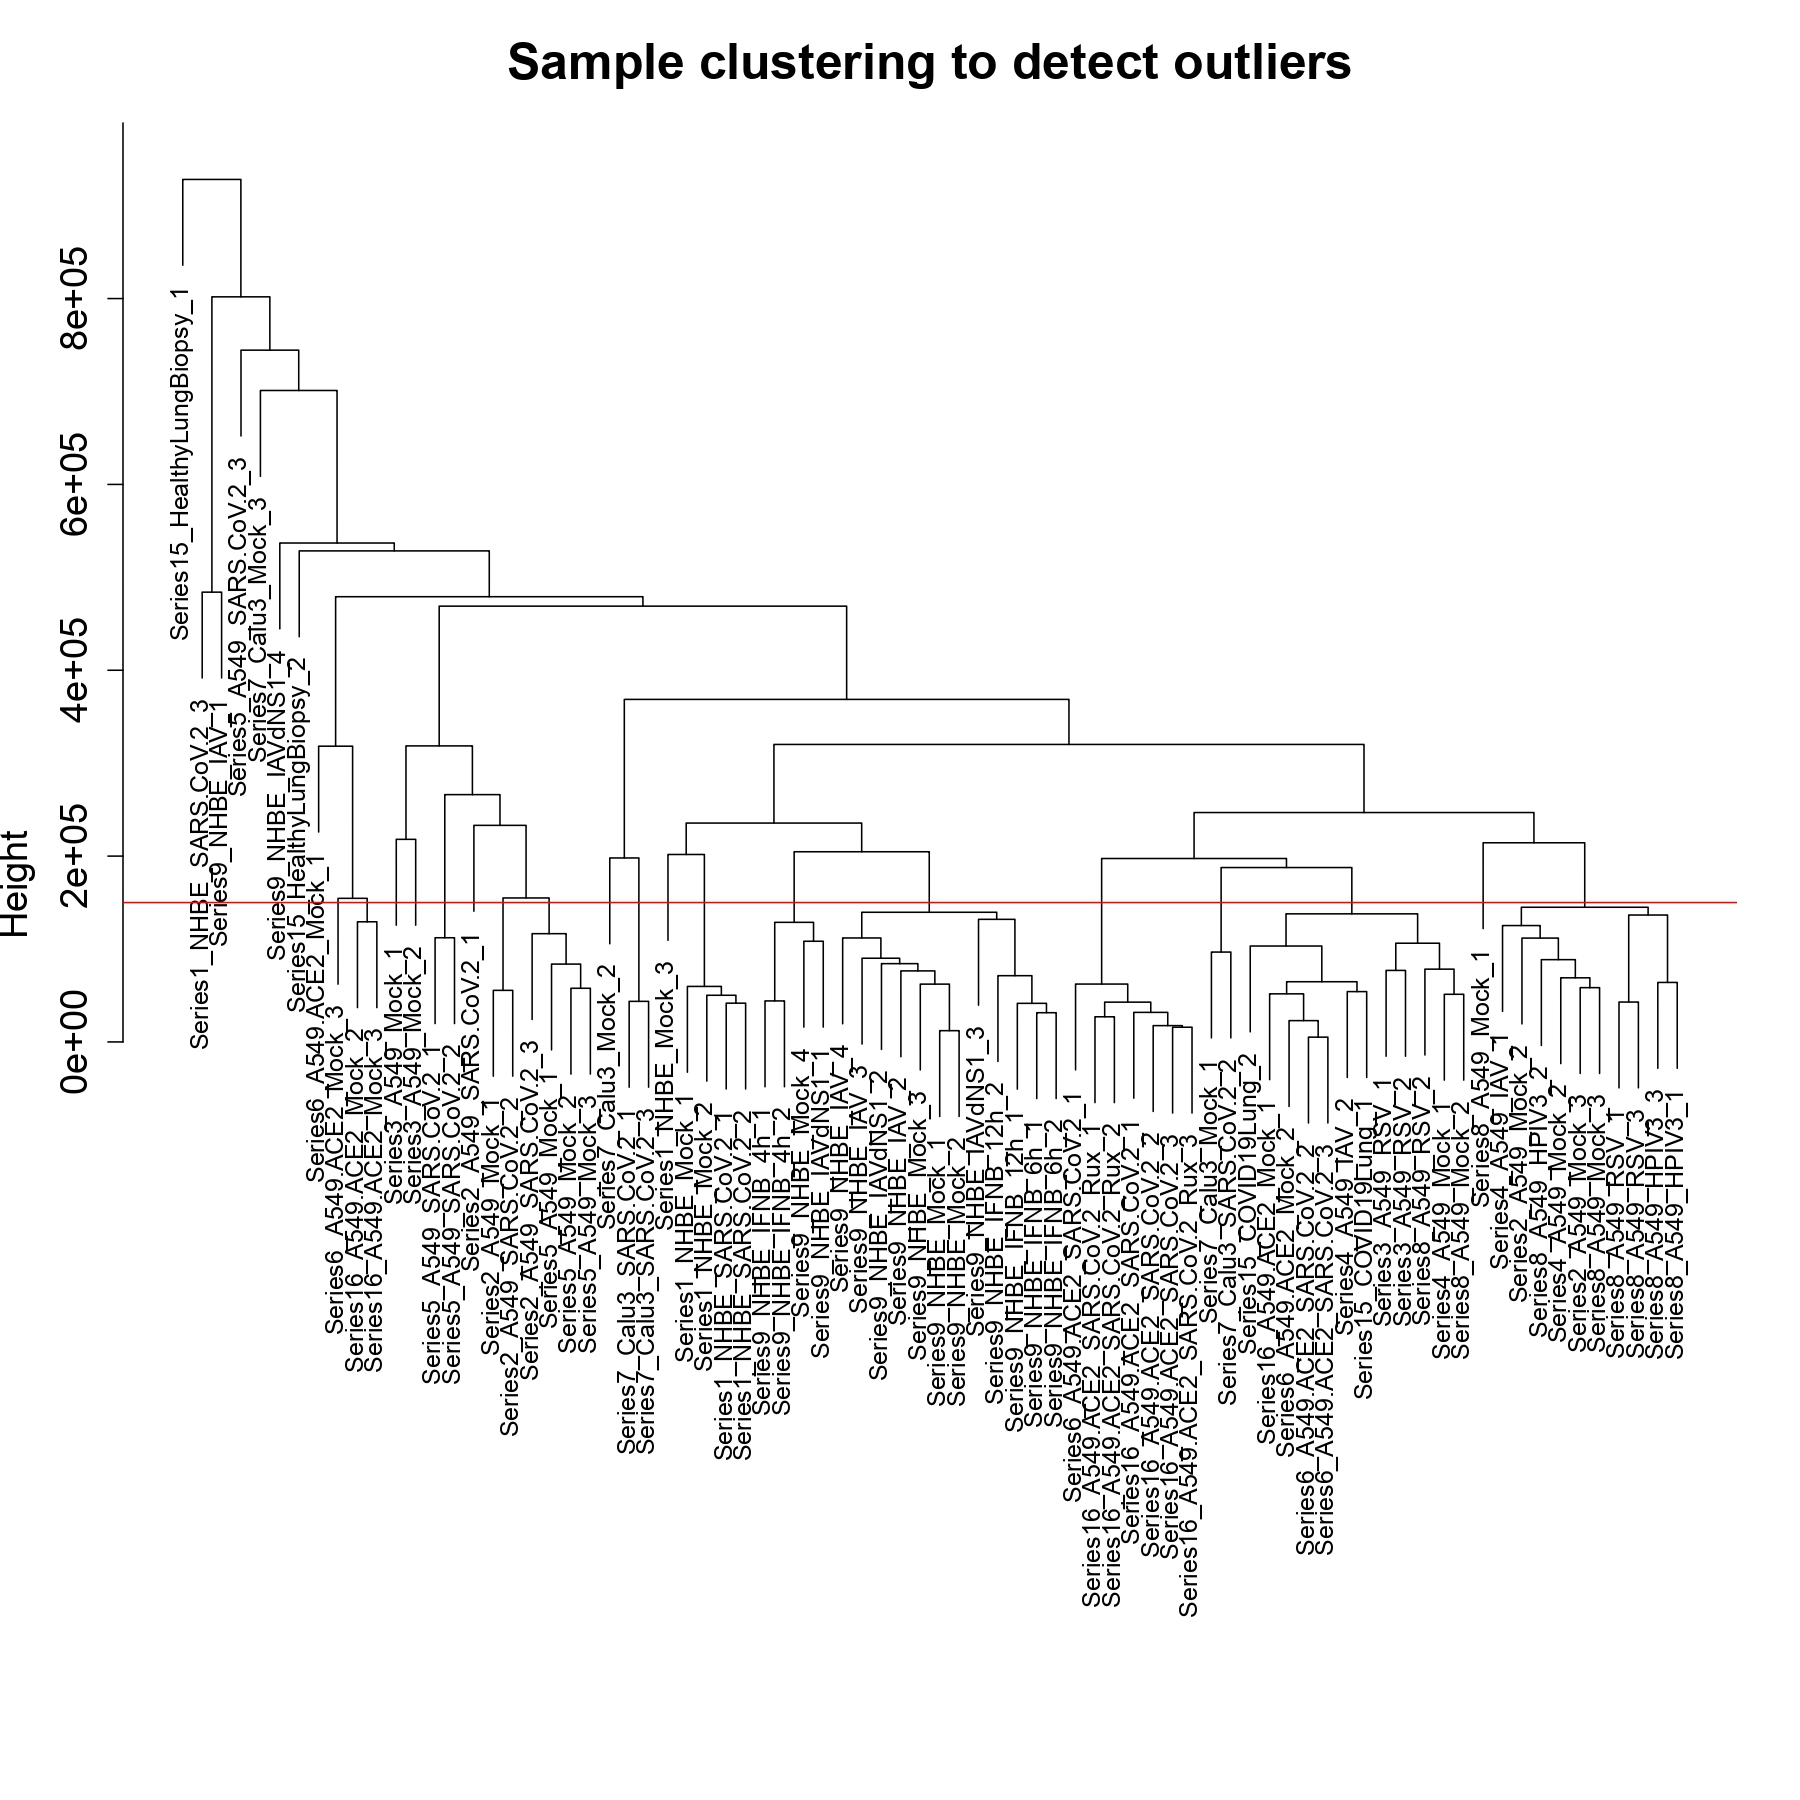
\includegraphics[width=0.9\textwidth]{figures/sampleClustering.jpg}}

\caption{Sample Clustering}
\label{fig:sample_clustering}
